\chapter{Architecture}

\section{General Overview}
\label{archi-intro}
There are three main ways in which we can see TCC at work. One could be what has been shown in the examples of the previous chapter: a client that want to purchase something and has to deal with a TCC-compliant service. In this case we would have a client extended with a TCC transaction manager and a server that can perform TCC transactions. A generalization of this concept brings a second possibility of implementing TCC: we can assume the transaction manager as a more general service that lays on the cloud, thus the client will only be extended to the point in which the transactions in progress will be dispatched to the transaction manager. When client is done and wants to confirm (or delete), it will dispatch the required actions to the transaction manager.\\
Finally, a third possibility is the interaction among servers, thus the client itself becomes a server and requires resources from another server in a TCC fashion.\\
During the development of my thesis, these dimensions were all explored. In this chapter we will see the architecture of the system; for the most part I show the views for the generalized TCC (with the transaction manager on the cloud) because it's the most interesting among all.

\section{Logical View}
\label{archi-tcc-logical-view}
The logical view of a system decomposes the system structure into software components and connectors. It's used to map functionality, use cases and requirements onto the components. It concerns functionality and it's target audience are primarily users and developers.\\

\begin{figure} [ht]
\centering
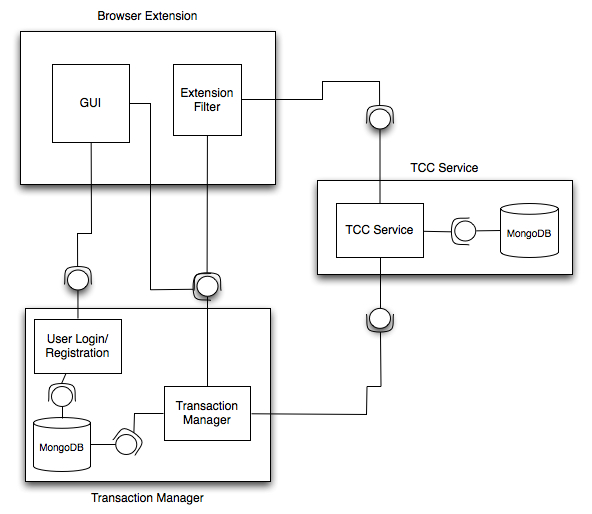
\includegraphics[scale=0.75]{images/logical_view.jpg}
\caption{Logical View of the system.}
\label{tcc-logical-view}
\end{figure}

The browser extensions has primarily two components: a GUI component which helps the user in tasks like logging in or registering into the transaction manager service and the extension filter. The task of the extension filter is to filter out confirmation links from HTTP headers received when reserving an item on a TCC service. As we can see the GUI component is directly connected to the login/registration component, which is used to register or log in into the transaction manager and to the transaction manager itself, to see current transactions in progress. It is not connected to the TCC service because it's not the GUI itself that dialogues with it, but the browser.\\
The TCC service is composed by a big homonym component and a MongoDB database. The component's task here is to work as any possibly service that offers resources, with the only difference that when a {\tt POST} request arrives for a resource, it does all the work to make it TCC compliant (explained in chapter \ref{chapter-tcc}). When answering with a confirmation link, the latter is intercepted (filtered) by the extension filter, which sends it to the transaction manager that will store it.\\
The transaction manager is composed by a small piece which deals with registrations and logins, and a big component which receives confirmation links and stores them. When questioned, the transaction manager component sends back the list of current transactions in progress to the GUI. When a confirmation request is asked by the GUI, the transaction manager confirms the transaction directly to the TCC service component using a {\tt PUT} request on the confirmation link.\\
For what concerns the logical view for an integrated transaction manager into the extension itself, this may turn as simply as a local storage for the extension that keeps track of the current transactions in progress. A registration/login component will not be needed since the transaction manager has to deal only with the transactions of the current user. In the case of servers interacting using TCC we have the same exact pattern except that the extension is not a browser extension per se but a server.

\section{Process View}
The process view models the dynamic aspects of the architecture: it defines which are the active components, which are the current threads of control, if there are multiple distributed processes in the system, what is the behavior of the various parts of the system and how all of them communicate. It concerns functionality and performance and the target audience are mainly developers.\\

\begin{figure} [ht]
\centering
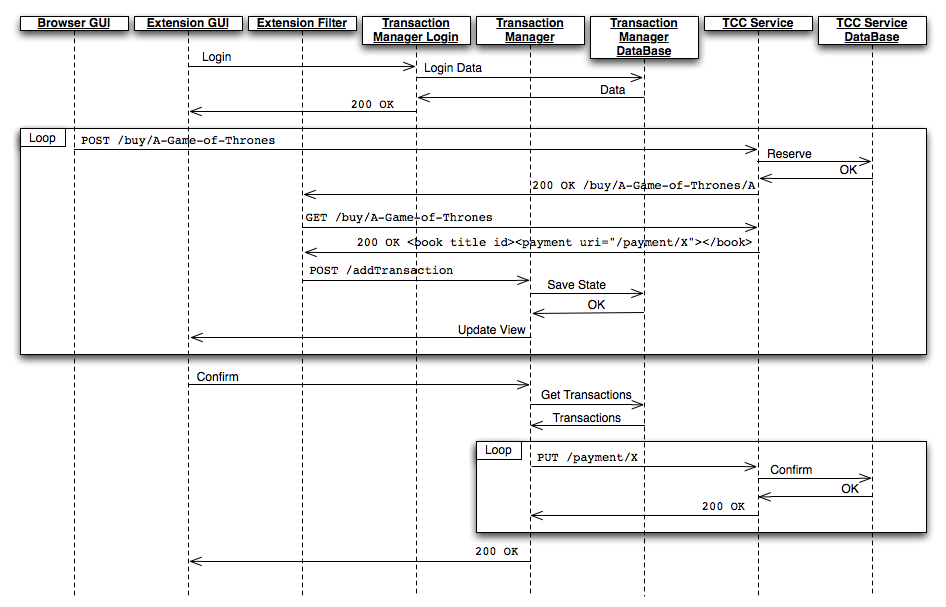
\includegraphics[scale=0.5]{images/process_view.jpg}
\caption{Process View of the system.}
\label{tcc-process-view}
\end{figure}

In figure \ref{tcc-process-view} we can see the previously described components in a general working flow. The first thing that we want to happen is the login from the extension to the transaction manager. Once this is done, the reservation loop can start. Basically what happens is that from the browser GUI, the user may {\tt POST} a reservation for an item. The TCC service sets the item as reserved, creates the resource and sends back the confirmation link to the browser. The link is subsequently intercepted by the extension filter, which does {\tt GET} on it to receive more information about the current transaction. As it receives them, they are sent to the transaction manager through a {\tt POST} request. The transaction manager stores them and updates the view that shows to the client the current transactions in progress.\\
This loop may go on for a while, the user may reserve as many items as he wants. When done, the user can confirm from the extension GUI the various transactions. A {\tt PUT} request is forwarded to the transaction manager, which gathers all the transaction for that user and starts a second loop that confirms, through a {\tt PUT} request on the various confirmation links, the transactions to the TCC service(s). Once done the transaction manager can notify the client that the confirmation happened successfully (or not).\\
As for what concerns the two variants of TCC, this workflow doesn't change. In the case of server interacting with another server there won't be any browser GUI, and if the transaction manager is local then login is not necessary either, but except for that the order of the actions and the actions done are the same.

\section{Development View}
The development view of a system is the static organization of the software code artifacts (for example packages, modules, binaries, etc.). Basically it maps the code with the logical view and it concerns reusability and portability. Target audience are usually developers.\\

\begin{figure} [ht]
\centering
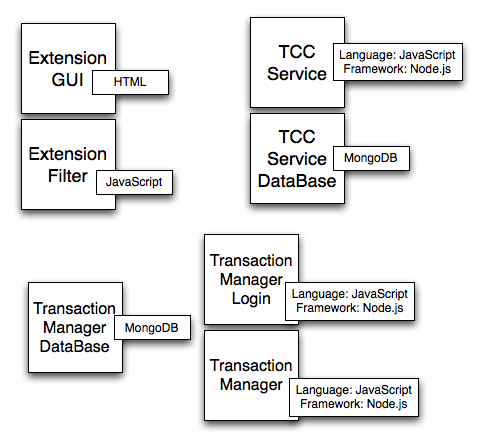
\includegraphics[scale=0.65]{images/development_view.jpg}
\caption{Development View of the system.}
\label{tcc-development-view}
\end{figure}

As we can see in figure \ref{tcc-development-view} for what concerns the browser extension, the GUI is done in plain HTML while the extension filter that intercepts the confirmation links is done in JavaScript. The service as well as the transaction manager are developed in JavaScript using as framework Node.js. Node.js is a server side framework to write servers in JavaScript. The choice of using it instead of any other framework in any other language was taken because creating a service with all the functionalities that were needed to implement TCC was very simple and straightforward. Same goes for the transaction manager and its functionalities. The two databases were implemented in MongoDB.\\
Of course any kind of choice regarding client and server sides is possible, given the correct implementation of the TCC protocol.

\section{Physical View}
The physical view defines the hardware environment (hosts, networks, storage, etc.) where the software will be deployed. Different hardware configurations may be used to provide different qualities. It concerns 	performance, scalability, availability, reliability and the target audience are operations.

\begin{figure} [ht]
\centering
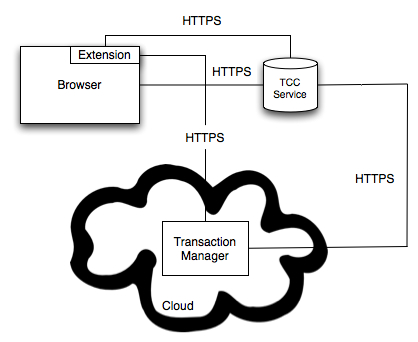
\includegraphics[scale=0.75]{images/physical_view.jpg}
\caption{Physical View of the system.}
\label{tcc-physical-view}
\end{figure}

As shown in figure \ref{tcc-physical-view}, HTTPS is the main channel through which communication is performed. I shall repeat that this configuration corresponds to the general TCC case described in \ref{archi-intro}. The browser can communicate to the TCC service with HTTP too, but when doing the {\tt POST} request, and receiving the result back (filtered by the extension), it's important that it's set to HTTPS, to avoid eavesdropping of the link. If the link gets eavesdropped, for an attacker it could be easy to confirm some reservations even if the reserver wants to cancel it afterwards. Same goes for the communication between the extension and the transaction manager (in which confirmation links are sent). As for the confirmation event we can assume that in the worst case, an attacker may want to intercept the various {\tt PUT} request, send back a bogus result and send a {\tt DELETE} to the confirmation link to cancel the transaction, instead of confirming it, thus again the use of HTTPS.\\
For what concerns a physical view for the other cases, again the use of HTTPS is encouraged to avoid man-in-the-middle attacks and eavesdropping if the protocol is used on a web-based service. As for the case in which different servers works on the same network or same machine, the use of a secure transfer protocol is highly suggested.

\section{Use Cases}
A use case is the specification of a set of actions performed by a system, which yields an observable result that is, typically, of value for one or more actors or other stakeholders of the system. The use cases this section is going to dive through will be useful to understand the flow of actions in the TCC protocol from the point of view of the user.\\
Note that these use case scenarios only describe the general TCC case, and do not explain the case in which the transaction manager is on the machine. This choice has been made because the general TCC case is also the most complicate in terms of elements in play, thus results more interesting to see.

\subsection{Immediate Purchase}
This use case explores the best case for user and for the sellers: a user performs a couple of reservations from the same website and confirms them right away. The service is happy because the user confirms as soon as possible, and the user is too because transactions won't timeout before he confirms them.\\
As pre-condition, the user should be registered to a transaction manager service that manages his transactions. There are no post-conditions.\\
Scenario: the user logs in into the transaction manager service using the browser extension installed in his browser. Then he starts navigating the website of a airline agency. He wants to book a flight composed of two connecting flights from two different airlines. In the first website, he finds the first flight and books it. As soon as the booking is completed, in the browser extension the reservation appears stating the name of the airline agency, the booked flight name and the remaining time to confirm the reservation.\\
Shortly later, the user moves to the second airline agency and finds eventually the second flight. After booking it, the reservation appears right after the first one in the browser extension. Now the user is assured that he will take those two flights, so he clicks on the confirmation button on the browser extension, that shortly after tells him that the transactions happened successfully.

\subsection{Deletion}
The following use case scenario explores the situation in which a user reserves something but doesn't find what he was searching for in another website. Since the purchase of only one of the two items he wanted to buy is meaningless, he deletes the order.\\
As pre-condition again, the user has to be registered to the transaction manager service. There are no post-conditions.\\
Scenario: the user logs in into the transaction manager service through the browser extension. First, he navigates to a website selling books: he wants to buy two books from the same fantasy series. In the current website he cannot find the first one, but manages to reserve the second one. In the browser extension now he can see his reservation. Later, he navigates to two different websites, but cannot find the first book of the series. Since he doesn't want to buy the second book without having the first one, he opens the browser extension and cancels the current transaction for the second book. The webstore makes the book available again and the user closes the pages.\\

\subsection{Timeout Before Confirmation}
In this use case scenario, the user will wait too much for confirming the reservations done. In this case the items will be available in the store again and he has to go through the reservation process once more to confirm them.\\
As for what concerns pre- and post-conditions they are the same of the previous scenario.\\
Scenario: the user logs in into the transaction manager service through the browser extension. Then navigates to a movie theater website. He wants to book a seat for a movie, and then book another seat for another movie right after the first one ended, in the same movie theater. The user easily finds both the movies and manages to reserve the two seats for the two movies. Right after he receives a phone call and forgets about the transaction in progress. He leaves the house. In the meantime transactions time out, the seats get available again and eventually all the seats for both shows get booked. As the user returns, he notices from the browser extension that the reservations are timed up, so he can't confirm them.

\subsection{Timeout During Confirmation}
This use case scenario explores the worst case, in which the user confirms some transactions but during confirmation some reservations time out so he end up having some transaction confirmed and some timeout.\\
As for what concerns pre- and post-conditions they are the same of the previous scenario.\\
Scenario: the user logs in into the transaction manager service through the browser extension. He navigates to three different webstores that sell PC components. On one of them he can find the best motherboards at the cheapest price, so he reserves one. On the second website he reserves two RAM banks and on the third one, he reserves the latest processor in terms of computing power. In the end he has on the browser extension three transactions with relative names and timeouts. After a while he decides to purchase and he realizes he has very few seconds left to confirm the transactions in progress. He decides anyway to confirm them. Some bad thing happens during the confirmation phase and some transaction got timeout before the confirmation arrives. The user ends up having bought two RAM banks and a processor but no motherboard.\\
Notice that this case is the \textit{heurstic exception} mentioned earlier, in the end of chapter \ref{chapter-tcc}. This is an unrecoverable state, so the user has to navigate back to the motherboard website and hope the motherboard he wants is not out-of-stock.\\

The next chapter will illustrate the components design and interface.